\section{Results}
\label{sec:results}

\section{Results for evolutionary approach 1}
\label{sec:results_1}

Like in section \ref{sec:challenges} already mentioned unstable simulation results and non-reproducibility were encountered which make it hard to interpret the results. Thus, good weights are interpreted mostly as weight with a high potential of a good reward. //
The same evolutionary algorithm was tested with slightly different configurations concerning hyper-parameters. 
The best distances of every generation were plotted with a logarithmic scale and can be seen in figure \ref{fig:results_1}. 

\begin{figure}[H]
	\centering
	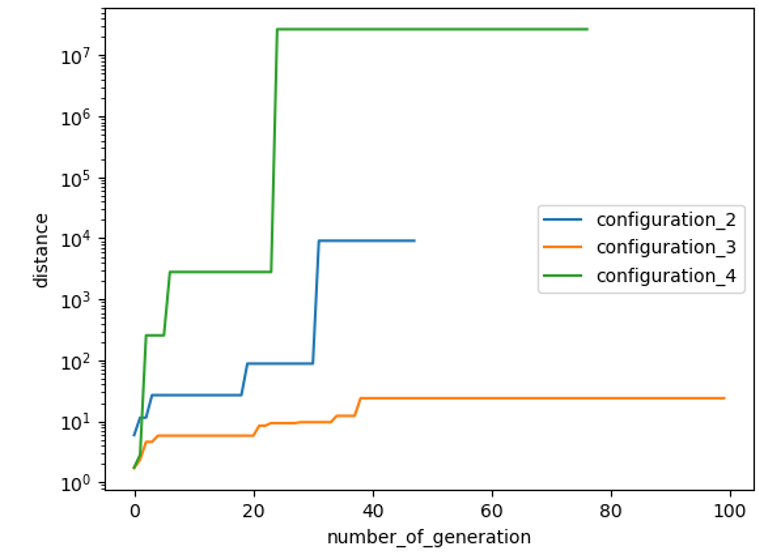
\includegraphics[width=3.3in]{img/results_1.png}
	\DeclareGraphicsExtensions.
	\caption{Results for different experiment configurations}
	\label{fig:results_1}
\end{figure}

In the first configuration a fixed input value was used and only 4 of the 7 output joints were controlled. ...
.
% TODO: als Liste machen !
\section{Conclusion}